\chapter{Authentication II: \texttt{SSO}\& \texttt{SAML}}
\label{chap:authentication-ii}
\thispagestyle{chapterInit}
Questo capitolo è dedicato all'approfondimento dell'autenticazione all'interno di internet, in particolare verrà trattato il concetto di \texttt{Single Sign-On} per la riduzione del numero di credenziali da memorizzare e la gestione di queste ultime. Inoltre verrà trattato il protocollo \texttt{SAML} ovvero \textit{Security Assertion Markup Language} per la gestione di autenticazioni e autorizzazioni tra domini diversi, infine si parlerà di \texttt{SPID}, \texttt{CIE} \& \texttt{eIDAS} come esempi di implementazioni a livello nazionale ed europeo di \texttt{SSO}.
\section{Single Sign-On (\texttt{SSO})}
    \label{sec:sso}
    Il concetto alla base per il \texttt{SSO} è quello di avere un'unica autenticazione per accedere a (quasi) tutti i servizi, per raggiungere questo scopo il fornitore di servizi (\texttt{SP}) demanda il processo di autenticazione ad una autorità di identità (\texttt{IdP}) che si occupa di verificare che l'utente sia chi dice di essere, tramite i meccanismi visti precedentemente nella sezione \ref{sec:user-authentication}\footnote{\nameref{sec:user-authentication}}, mentre il processo di \textit{outsourcing} del processo di autenticazione è stato trattato nella sezione \ref{sec:outsourcing-authentication} \footnote{\nameref{sec:outsourcing-authentication}}.
    \paragraph{Funzionamento} Il funzionamento di un sistema \texttt{SSO} è il seguente:
        \begin{enumerate}
            \item L'utente accede all'applicazione \texttt{SP}
            \item L'applicazione \texttt{SP} reindirizza l'utente all'\texttt{IdP} per il processo di autenticazione
            \item L'\texttt{IdP} in primo luogo chiede all'utente di autenticarsi, il quale fornisce le proprie credenziali e l'\texttt{IdP} verifica l'identità dell'utente
            \item L'\texttt{IdP} genera un \textit{token} che viene cifrato e firmato con la chiave privata dell'\texttt{IdP} e inviato all'applicazione \texttt{SP}
            \item L'applicazione \texttt{SP} verifica la firma del \textit{token} con la chiave pubblica dell'\texttt{IdP} e se la verifica è positiva lo considera valido e lo inoltra all'utente che lo utilizzerà per accedere ai servizi (includendolo nelle richieste)
        \end{enumerate}
        Questo è il processo che avviene usualmente ma è possibile che il \textit{token} venga inviato all'utente dell'\texttt{IdP} e non direttamente all'applicazione del \texttt{SP}. In questo caso l'utente verifica la firma del \textit{token} con la chiave pubblica dell'\texttt{IdP} e poi lo includerà nelle richieste ai servizi.
    \paragraph{Proprietà} Le principali proprietà e vantaggi di un sistema \texttt{SSO} includono: la conservazioni delle credenziali in un unico posto e il non trasferimento delle stesse ad ogni servizio, i \textit{service provider} devono fidarsi dell'\textit{identity provider} nel verificare l'identità dell'utente. Inoltre il processo di autenticazione deve essere protetto, questo scopo lo si raggiunge usando la crittografia a chiave pubblica \footnote{ vedi \nameref{sec:PKI}} e con meccanismi di firma digitale.
    In questo paradigma è importante che l'\texttt{IdP} sia affidabile e che sia in grado di proteggere la \textit{confidentiality} e l'\textit{integrity} dei dati, inoltre è importante che l'\texttt{IdP} rimanga disponibile in quanto questo è un cosiddetto \textit{single point of failure}.
\section{Security Assertion Markup Language (\texttt{SAML})}
    \texttt{SAML} è un paradigma di autenticazione standard che sfrutta il formato \texttt{XML} per lo scambio di informazioni, questo lo rende molto \textit{verbose} anche per una piccola porzione di dati. Questo standard è stato introdotto nel 2002 e aggiornato nel 2005 in risposta alla mancanza di standard per lo scambio di informazioni di autenticazione e autorizzazione tra domini diversi.
    
    \begin{wrapfigure}{r}{0.25\textwidth}
        \centering
        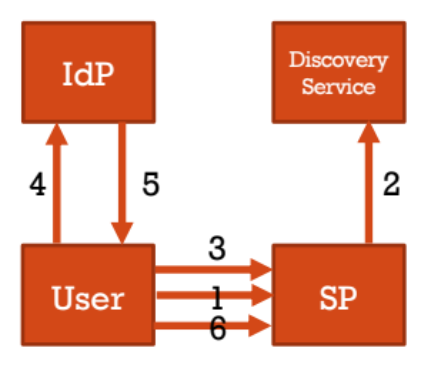
\includegraphics[width=0.25\textwidth]{05/SAML-Auth.png}
        \caption{Esempio di utilizzo di \texttt{SAML}}
    \end{wrapfigure}
    \paragraph{Esempio d'uso di \texttt{SAML}} In uno scenario dove ad esempio per avere uno sconto sul noleggio di un'auto è necessario essere membri VIP di una compagnia aerea, allora un utente (\textit{alice}) eseguirà il login sul sito della compagnia aerea (che agisce da \texttt{IdP} e \texttt{SP}) e poi verrà reindirizzata al sito di noleggio auto (che agisce solo da \texttt{SP}) con le informazioni dello status VIP dell'utente. A questo punto \textit{alice} può ottenere lo sconto da parte del sito di noleggio auto anche senza essersi autenticata su quest'ultimo, in quanto valgono le informazioni inviate dal sito della compagnia aerea.\newline
    In breve:
        \begin{enumerate}
            \item L'utente vuole accedere ad un servizio \texttt{SP}
            \item Questo servizio \texttt{SP} reindirizza l'utente ad un \textit{Discovery Service} che permettere all'utente di scegliere l'\texttt{IdP} per l'autenticazione
            \item Dopo essersi registrato tramite il \texttt{IdP} scelto l'utente torna al servizio \texttt{SP} con una identità valida verificato da un \texttt{IdP}
            \item Allora il fornitore di servizi rimanda l'utente al suo \texttt{IdP} per ottenere un \textit{token} di autorizzazione
            \item L'utente si autentica sul \texttt{IdP} e ottiene un \textit{token} di autorizzazione
            \item L'utente ritorna al servizio \texttt{SP} con il \textit{token} di autorizzazione e può accedere ai servizi
        \end{enumerate}
    
    \subsection{\texttt{SAML} Overview}
        Come mostrato in figura \ref{fig:saml-overview} l'architettura di \texttt{SAML} è composto da diversi componenti quali:
        \begin{description}
            \item[\textit{Assertions}] - Le dichiarazioni fatte dal \texttt{IdP} riguardo l'identità dell'utente
            \item[\textit{Protocols}] - I protocolli usati per lo scambio di informazioni tra i vari componenti
            \item[\textit{Bindings}] - I meccanismi usati per associare i protocolli di \texttt{SAML} con i protocolli di comunicazione
            \item[\textit{Profiles}] - La combinazione di \textit{Assertions}, \textit{Protocols} e \textit{Bindings} a supporto di uno specifico caso d'uso
            \item[\textit{Authentication Context}] - Un dettaglio sui tipo di autenticazione e livello di sicurezza
            \item[\textit{Metadata}] - Dati di configurazione per \texttt{IdP} e \texttt{SP}
        \end{description}
        \begin{figure}[H]
            \label{fig:saml-overview}
            \centering
            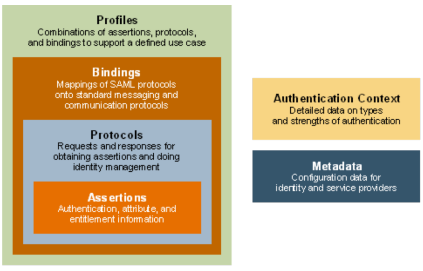
\includegraphics[width=0.5\textwidth]{05/SAML-Overview.png}
            \caption{Overview di \texttt{SAML}}
        \end{figure}
        \subsubsection{\textit{Assertions}}
            Le \textit{Assertions} sono le dichiarazioni fatte da una \texttt{SAML} \textit{authority} detta anche "parte dichiarante" (\textit{asserting party}). Le assertions possono essere viste come le unità di informazione di \texttt{SAML} e sono divise in tre tipi:
            \begin{description}
                \item[\textit{Authentication Assertion}] - Rilasciato dalla parte che autentica l'utente, contiene informazioni quali: chi ha autenticato l'utente, chi è il soggetto autenticato, quando è valida l'autenticazione, ecc\dots
                \item[\textit{Attribute Assertion}] - Contiene informazioni sullo stato dell'utente, come nell'esempio di \textit{alice} l'appartenenza al programma VIP
                \item[\textit{Authorization Assertion}] - Contiene informazioni su cosa può fare l'utente, come ad esempio la possibilità di noleggiare un'auto quando in viaggio di lavoro
            \end{description}
            \paragraph{\textit{Authentication Assertion}}
                Questo tipo di \textit{assertion} è strutturato nel seguente modo:
                \begin{description}
                    \item[Intestazione] - Contiene informazioni sulla versione di \texttt{SAML} usata, lo schema per \texttt{XML} e l'ora di creazione (\textit{issue instant})
                    \item[Autorità] - Contiene informazioni sul \texttt{IdP} che ha rilasciato l'\textit{assertion}
                    \item[Soggetto] - Contiene un identificativo univoco che rappresenta l'utente autenticato
                    \item[Condizioni] - Contiene informazioni sulla validità dell'\textit{assertion} (vale non prima di, non dopo il) con data e ora
                    \item[\textit{Authenticating Context}] - Contiene informazioni sul tipo di autenticazione e il livello di sicurezza che è stato usato\footnote{Si noti come la autenticazione in se non è parte del \texttt{SAML}, nelle \textit{assertion} ci si riferisce ad un processo di autenticazione avvenuto precedentemente}
                \end{description}
            \paragraph{\textit{Attribute Assertion}}
                Questo tipo di \textit{assertion} è strutturato nel seguente modo:
                \begin{description}
                    \item[Intestazione] - Contiene informazioni sulla versione di \texttt{SAML} usata, lo schema per \texttt{XML} e l'ora di creazione (\textit{issue instant}) l'unica differenza con l'\textit{Authentication Assertion} è il tipo di schema usato
                    \item[Attributo] - Contiene un identificatore del tipo di attributo (solitamente in modo molto specifico) e il valore dell'attributo
                \end{description}
        \subsubsection{\textit{Protocols}}
            I protocolli sono i meccanismi usati per lo scambio di asserzioni tra le varie parti e descrivono come poterne ottenerne una, come usarla e come verificarla. Vengono definiti anche protocolli sulle richieste di autenticazione e sulla risoluzione di parametri "passati per riferimento", viene definito anche un protocollo per il \textit{single logout} e per la gestione delle sessioni, e molo altro\dots\newline
            Distinguiamo come protocolli di comunicazione quei sistemi che permettono a due o più entità di scambiarsi informazioni definendo regole, semantica, sintassi e sincronizzazione. Esistono inoltre i protocolli di criptografia che sono designati alla protezione della comunicazione tra due entità, vengono applicati usando i \textit{cryptographic primitives} (come funzioni di \textit{hash}, cifrature simmetriche e asimmetriche, ecc\dots).
        \subsubsection{\textit{Bindings}}
            I \textit{bindings}, come anticipato, sono i meccanismi usati per definire i meccanismi per il trasporto dei messaggi \texttt{SAML} su protocolli di comunicazione diversi, come ad esempio \texttt{SAML URI}, \texttt{SAML SOAP}, \texttt{HTTP Redirect}, \texttt{HTTP POST}, ecc\dots
            \paragraph{\texttt{HTTP Redirect}} Questo meccanismo, in particolare, permette la trasmissioni di messaggi \texttt{SAML} tramite parametri di \texttt{URL} in una richiesta. In questo modo viene usato lo \textit{UserAgent} come intermediario per la trasmissione dei messaggi, questo meccanismo potrebbe essere necessario se è richiesta l'interazione con l'utente per generare una risposta. Questo è di gran lunga il meccanismo più usato (oltre che il preferito) per la trasmissione di messaggi \texttt{SAML} e per il \textit{SSO}.